V této kapitole si popíšeme, jaký je vlastně aktuální stav běžícího systému, a vysvětlíme si, co je potřeba pro přidání nového modulu.

\section*{Verzování a nasazení}

Pro verzování zdrojových kódů svých služeb jsem se rozhodl využívat GitHub~\cite{GitHubExplanation}, což mi umožňuje efektivně zálohovat kód.
V rámci GitHubu používám GitHub Workflow, které automatizuje proces vytváření Docker image~\cite{GitHubActionsDocker}, což zrychluje a automatizuje proces nasazení nové verze služby.
Jakmile je Docker image vytvořen, nahrávám jej na platformu Docker Hub\cite{DockerHub}.
Na tuto platformu image ukládám a následně je vzdáleně načítám při nasazení konkrétní služby.

\section*{Infrastrukturní přípravné práce}

Vlastní instalaci částí systému Coopmaster do kurníku a výběhu předcházely přípravné stavební práce.
Do budovy bylo třeba přivést Ethernetové připojení, což nebyl vůbec snadný úkol.
Dále pak bylo potřeba připravit a nainstalovat rozvaděč s řídící elektronikou
(obrázky~\ref{fig:instalace_rozvadec_krabice}~\ref{fig:instalace_rozvadec_vyzbroj}).
Musel jsem také na příslušných místech udělat průrazy zdí, v místech kde povedou kabely z rozvaděče ke kamerám a do kurníku.
Samotné Ethernetové připojení jsem vyřešil poněkud nestandardně.
Nepřicházelo v úvahu, abych táhl metalický kabel od domácího routeru do chléva, kvůli přílišné náročnosti na stavební úpravy.
Použil jsem tedy Wifi extender s Ethernet výstupem a elektroniku v kurníku jsem k internetu připojil přes něj.

\begin{figure}[H]
    \centering
    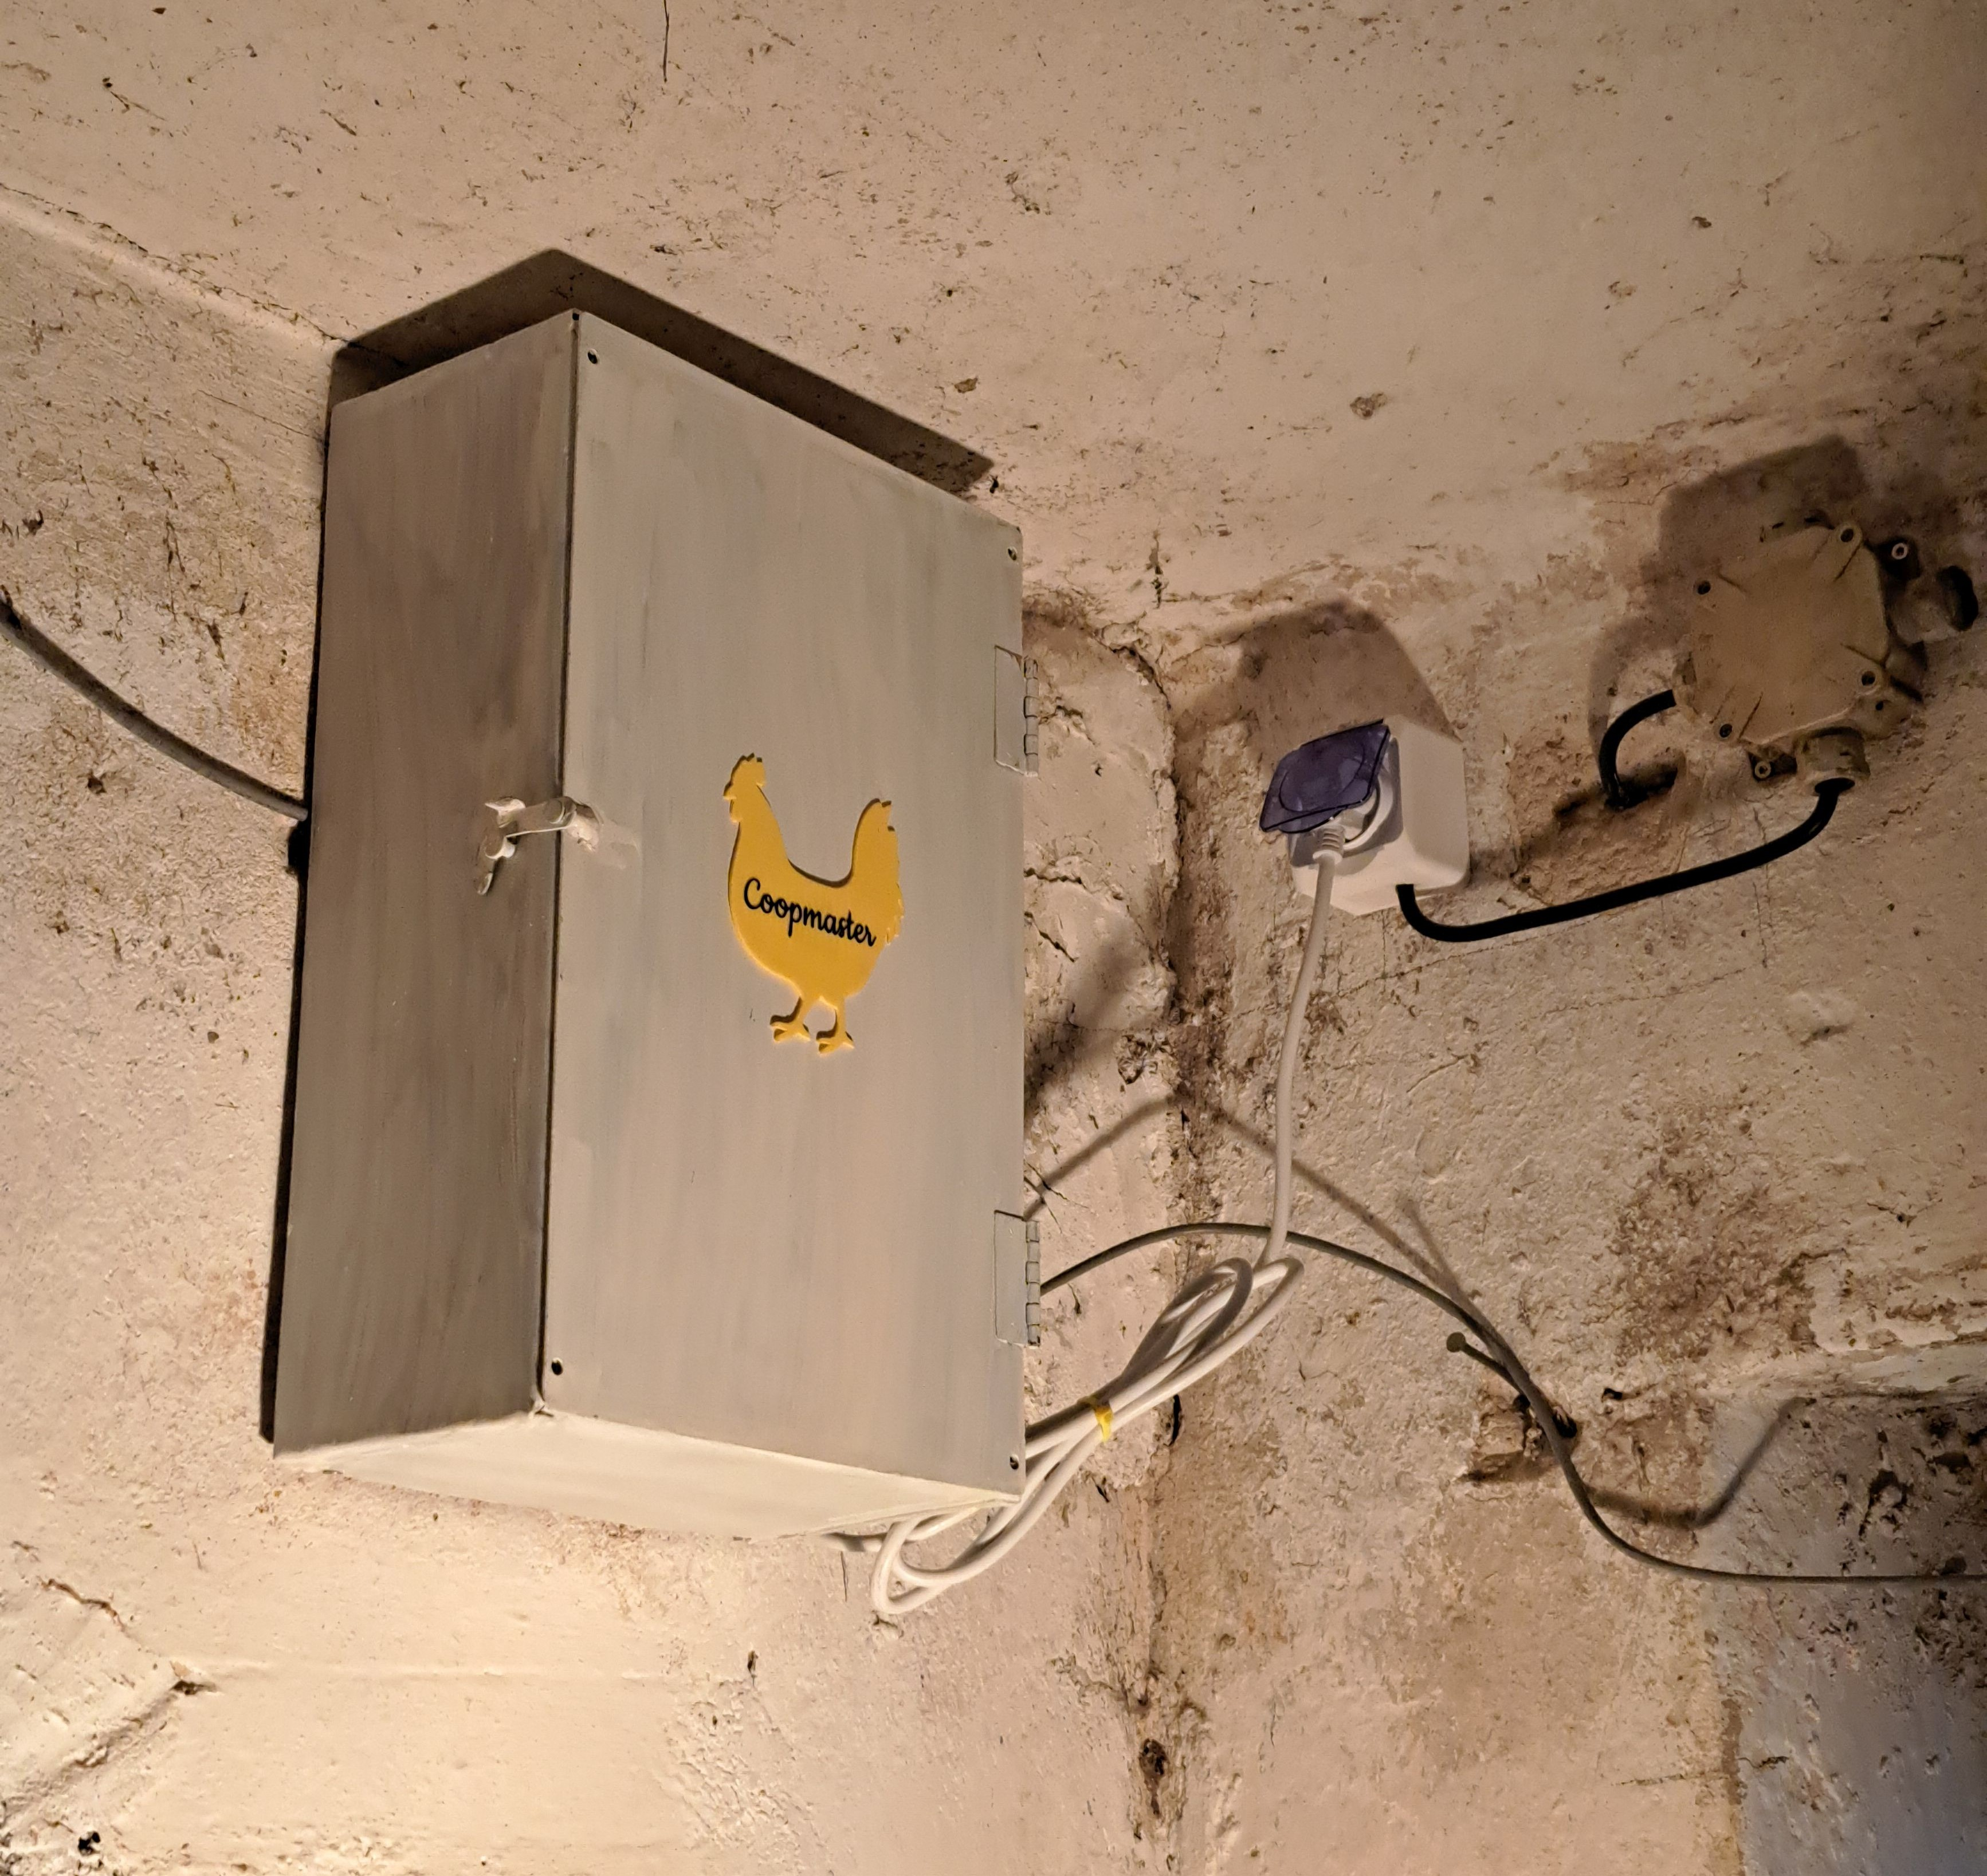
\includegraphics[width=0.8\textwidth]{img/instalace_rozvadec_krabice}
    \captionAuthorSource{Nainstalovaný rozvaděč ve chlévě}
    \label{fig:instalace_rozvadec_krabice}
\end{figure}
\begin{figure}[H]
    \centering
    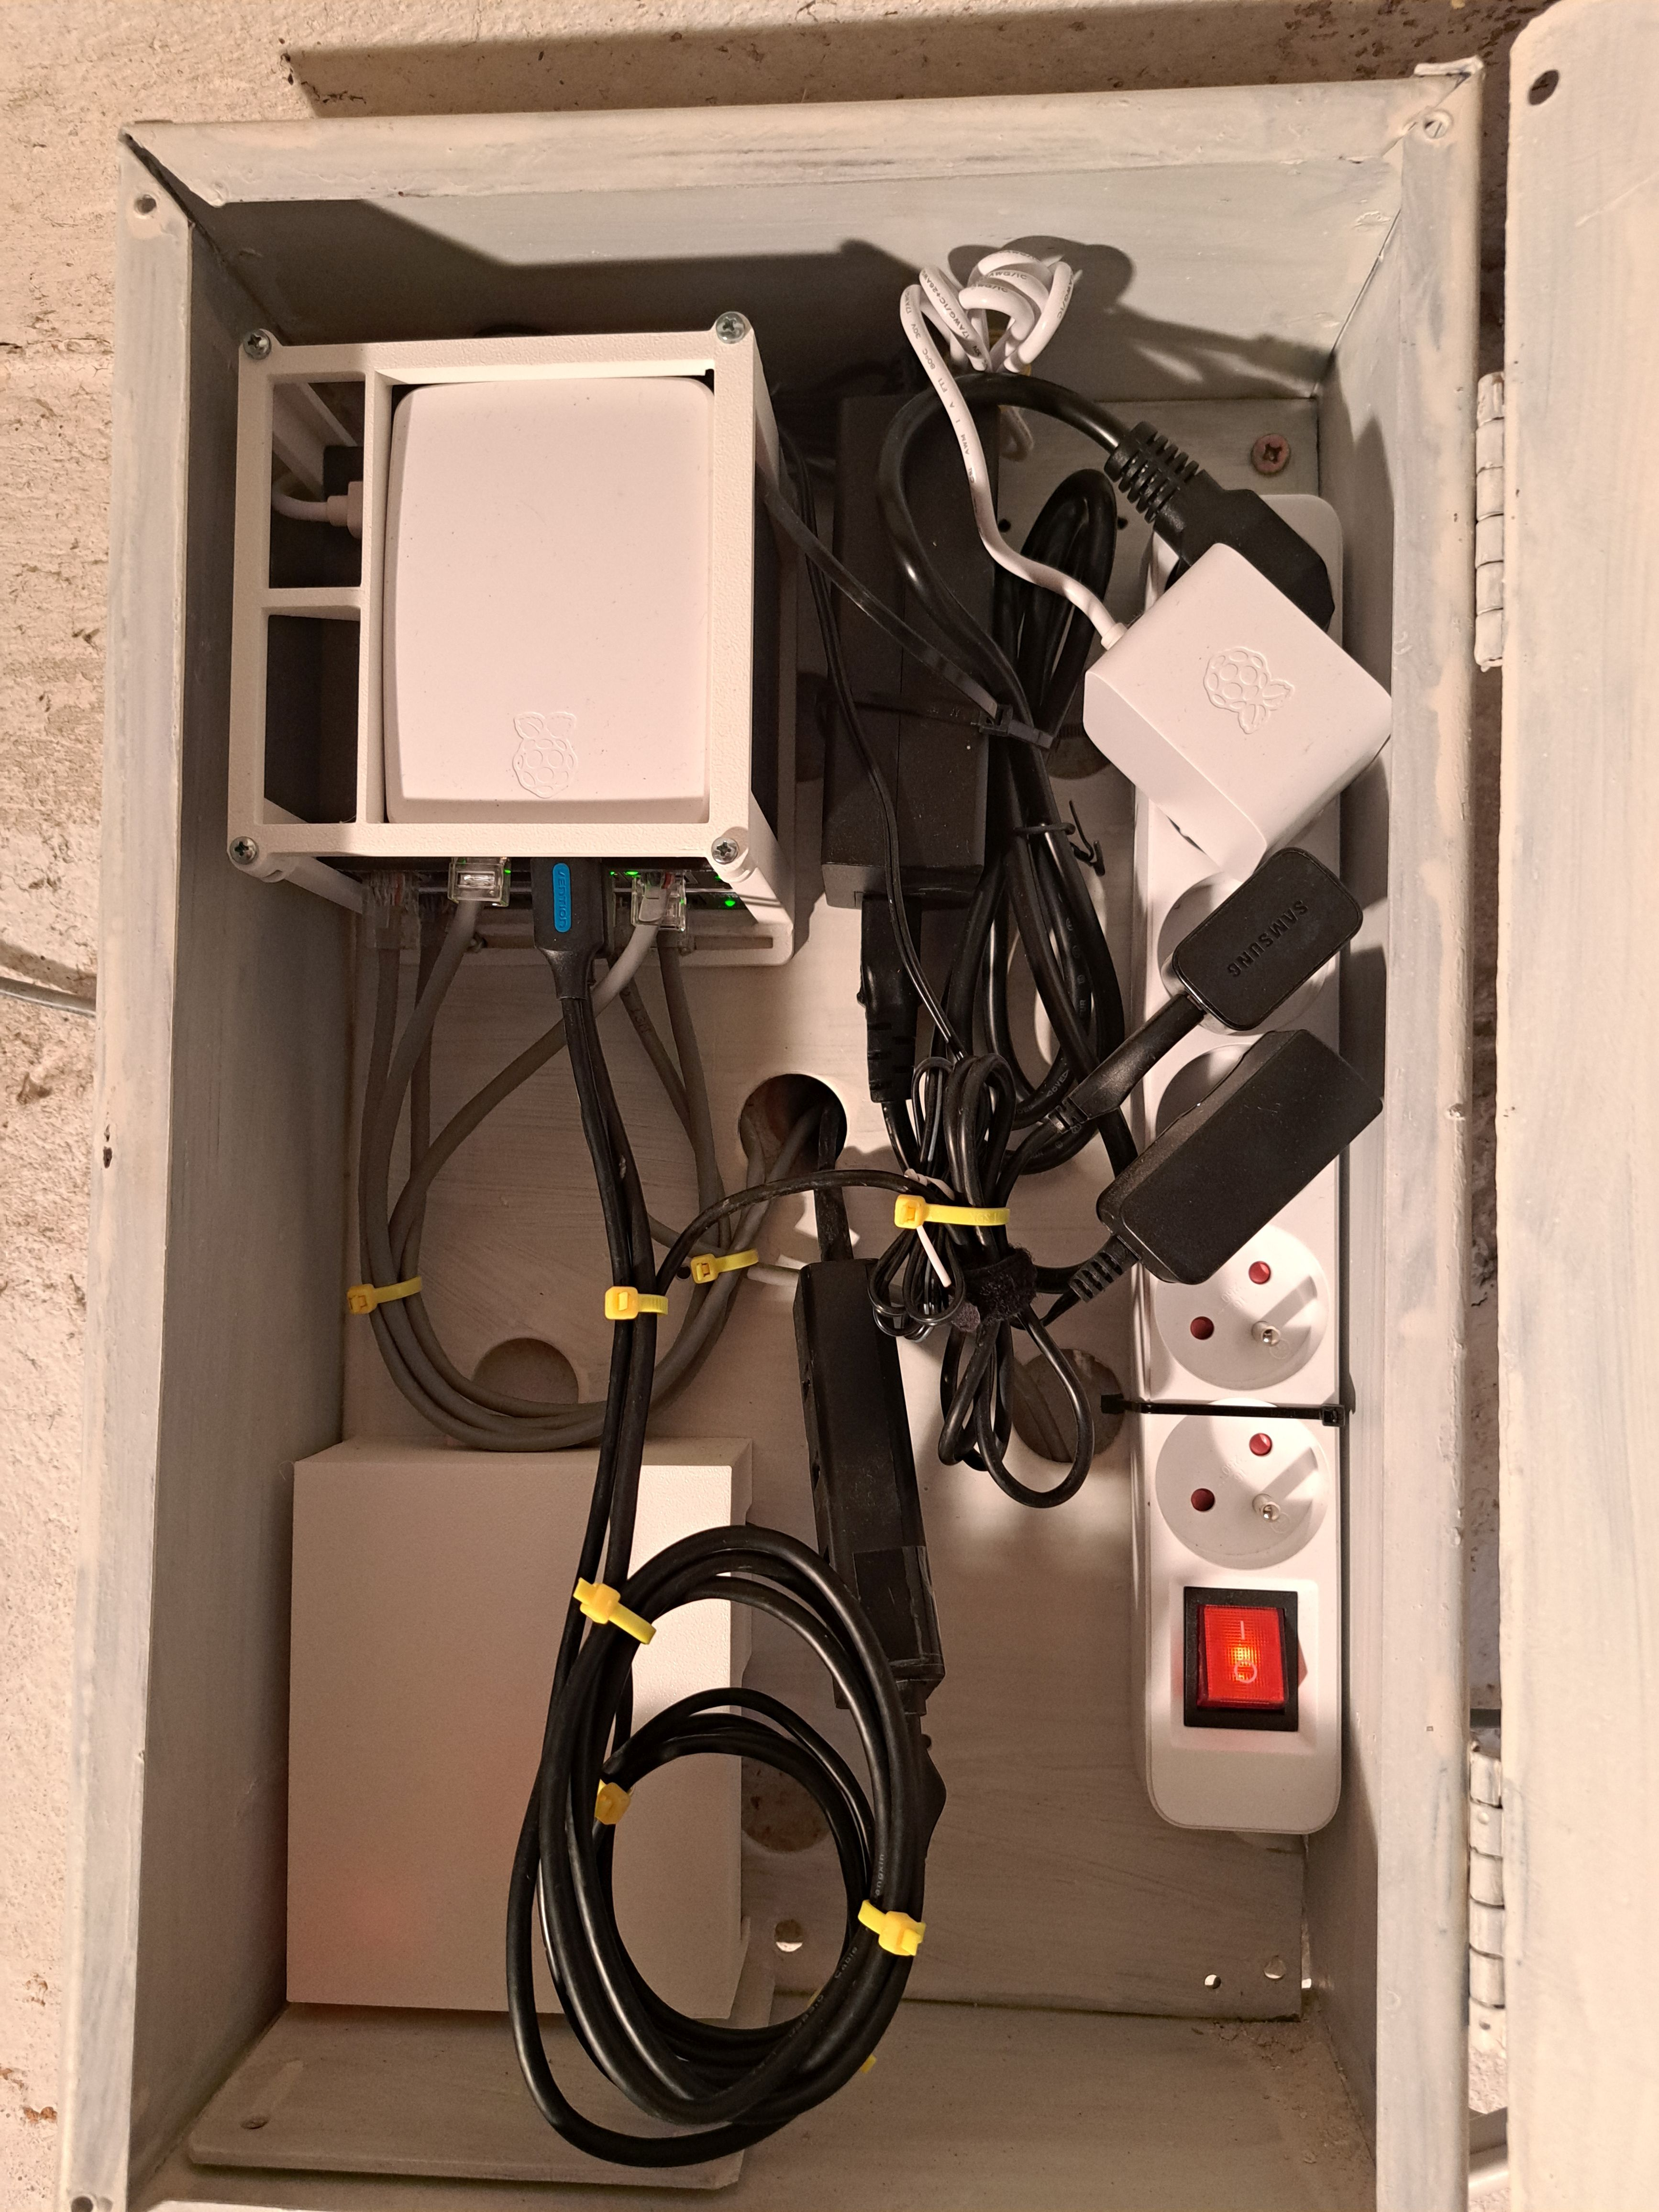
\includegraphics[width=0.8\textwidth]{img/instalace_rozvadec_vyzbroj}
    \captionAuthorSource{Vnitřek rozvaděče}
    \label{fig:instalace_rozvadec_vyzbroj}
\end{figure}

\section*{Výsledná fyzická infrastruktura}

Doma v místnosti se stabilním prostředím, které je vhodné pro výpočetní techniku, běží Intel NUC 11~\cite{IntelNUC11Enthusiast} s operačním systémem Ubuntu 22.04 LTS.
Tento počítač slouží jako hlavní server a zdroj výpočetního výkonu pro neuronové sítě.
Výpočetní výkon je poskytnut díky grafické kartě NVIDIA GeForce RTX 2060.\newline
Dále pak máme v kurníku a ve výběhu periferie (dvířka, senzory a kamery), které potřebují propojit se systémem Coopmaster.
Všechny tyto periferie jsou do systému připojeny skrze mikropočítač Raspberry Pi 5~\cite{RaspberryPi5} s operačním systémem Ubuntu 24.04 LTS.
Výpočetní část je takto rozdělena do dvou částí kvůli agresivnímu prostředí v kurníku (vlhkost, teplotní výkyvy).
Raspberry Pi 5 je mnohem levnější než Intel NUC 11 a v případě poškození zařízení vlivem prostředí, nevznikne tak velká škoda.
Síťová komunikace je mezi těmito dvěma počítači realizována pomocí služby Tailscale~\cite{Tailscale}, která mezi nimi vytváří mesh VPN.
Zároveň této služby využívám já jako správce, abych měl vzdálený přístup k oběma zařízením.

\section*{Základní konfigurace a klíčové služby}


Systém je rozvržen tak, že na počítači v kurníku běží služby, které zajišťují komunikaci mezi hardwarovými periferiemi a dalšími službami systému Coopmaster.
Doma na počítači jsou služby, jež potřebují výpočetní výkon a řeší konkrétní body zadání.
Na obou počítačích musí tedy být nainstalovaný Docker společně s nástrojem Docker Compose, aby bylo možné služby hromadně spouštět a konfigurovat.
Parametry jednotlivých služeb se načítají v obou případech ze souboru .env, aby konfigurační soubor Docker Compose neztrácel na přehlednosti.\newline

Základní služby, které jsou nutným minimem pro fungování systému, jsou
\begin{itemize}
    \item Home Assistant (\ref{sec:home-assistant})
    \item Postgres 15 (\ref{sec:postgres-15})
    \item Eclipse Mosquitto (\ref{sec:eclipse-mosquitto})
    \item Health Checker (\ref{sec:health-checker})
    \item Cloudflared (\ref{sec:cloudflared})
\end{itemize}
Tyto služby tvoří běhové prostředí, do kterého jsou již pouze zasazovány jednotlivé moduly systému Coopmaster.

\section*{Procedura přidání nového modulu}


Nyní si ukážeme celý proces, jak přidat do systému Coopmaster nový modul.
Ukázku provedeme na modulu pro detekci vetřelců.
Máme tedy dvě služby Camera Driver a Dog Alarm, tedy jedna služba pro poskytování dat a druhá pro výpočty.\newline

Například tento modul využívá data z IP kamery ve výběhu, kterou je zde potřeba nainstalovat, nakonfigurovat a připojit na Ethernet.\newline

Následně je třeba do Docker Compose konfigurace v kurníku přidat službu, která bude data z kamery předávat do útrob systému Coopmaster.
Této službě je třeba nastavit parametry na základě nichž bude fungovat.
V aktuální situaci je tato služba Camera Driver a vyžaduje IP adresu a přihlašovací údaje k IP kameře.\newline

Jakmile připojíme novou periferii pomocí driver služby do systému, potřebujeme službu, která data zpracuje.
Tato služba se musí přidat do Docker Compose konfigurace běžící doma na počítači Intel NUC 11 a opět jí musíme nastavit požadované parametry.
Každá služba z výpočetní sekce vyžaduje minimálně přihlašovací údaje a IP adresu MQTT brokeru.
V tomto případě se jedná o službu Dog Alarm, která se stará o detekci vetřelců na záběrech kamery.
Jako parametry tato služba vyžaduje zmíněné údaje o MQTT brokeru a dále pak IP adresu a port služby, ze které má stahovat obrázky k analýze.\newline

Služby z výpočetní části posílají výsledky své činnosti skrze MQTT broker do systému Home Assistant, aby je zobrazil.
Aby Home Assistant věděl, jak má s daty pracovat, je třeba ho nakonfigurovat pomocí souboru configuration.yaml.
Do tohoto souboru se definují entity, které představují jednotlivé vstupní a výstupní prvky.
Zde se jedná o několik MQTT entit.
Každé definujeme minimálně název, topic a datový formát.\newline

Na závěr je třeba pomocí webového rozhraní systému Home Assistant přidat karty a automatizace, které budou vizualizovat a reagovat na data přijatá do entit.
Pro tento modul je potřeba hned několik karet, a to kartu pro vizualizaci fotografií z kamery, kartu pro upozornění chovatele na hrozbu.
Je třeba také přidat automatizaci, která odešle chovateli notifikaci o hrozícím nebezpečí.\newline

Pro shrnutí můžeme říci, že jsme si popsali kompletní proces přípravy, přidání, konfigurace a nasazení nového modulu do ekosystému Coopmaster.



